\documentclass[tikz,12pt]{standalone}
\usetikzlibrary{shapes,arrows,positioning}
\definecolor{brewred}{RGB}{228,26,28}
\definecolor{brewblue}{RGB}{55,126,184}
\definecolor{brewgreen}{RGB}{77,175,74}

\usepackage{helvet}
\renewcommand{\familydefault}{\sfdefault}

\begin{document}
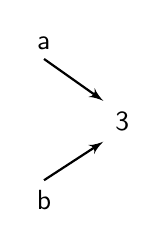
\begin{tikzpicture}[node distance=4em]
  \tikzset{
    value/.style={draw=none},
    binding/.style={draw=none},
    myarrow/.style={->, >=latex', shorten >=1pt, thick},
  }

  \node[value] (int) {3};
  \node[binding] (a) [above left of=int]{a};
  \node[binding] (b) [below left of=int]{b};

  \draw[myarrow] (a.south) -- (int.north west);
  \draw[myarrow] (b.north) -- (int.south west);

\end{tikzpicture}
\end{document}
